\section{Results}

\begin{table*}[t]
\centering
\footnotesize
\setlength{\tabcolsep}{2.6pt}
\caption{nDCG@10 for reranking the BM25 top-100 (Pyserini runs and qrels, as in RankGPT/RankLLM). $^\uparrow$/$^\downarrow$: significantly better/worse than bge-reranker-v2-m3 (paired $t$-test over queries, Holm-corrected over the collections each pair was evaluated on, $p<0.05$). Best displayed configuration per column in bold; all formats and controls appear in Appendix Table~\ref{tab:ranking-full}. Averages are reported only for systems run on every collection of the group (dash otherwise); matched comparisons for Clef and the P(yes) LLMs are given in the text. Touche, News and Robust04 contain long documents that every model truncates (Table~\ref{tab:longdoc}).}
\label{tab:ranking}
\begin{tabular}{lrrrrr|r|rrrrrrrr|r|r}
\toprule
 & \multicolumn{6}{c|}{TREC Deep Learning} & \multicolumn{9}{c|}{BEIR} & \\
System & DL19 & DL20 & DL21 & DL22 & DL23 & \textit{Avg} & Covid & NFC & Touche & DBP & SciF & Signal & News & Rob04 & \textit{Avg} & \textbf{All} \\
\midrule
BM25 (first stage) & 50.6 & 48.0 & 44.6 & 26.9 & 26.2 & 39.3 & 59.5 & 32.2 & \textbf{44.2} & 31.8 & 67.9 & 33.1 & 39.5 & 40.7 & 43.6 & 41.9 \\
\addlinespace[1pt]
\multicolumn{17}{l}{\textit{Cross-encoders}} \\
MiniLM-L6 (22M) & 72.7 & 67.5 & 65.6 & 49.9 & 42.2 & 59.6 & 74.5 & 34.9 & 28.4$^\downarrow$ & 43.9 & 69.5$^\downarrow$ & \textbf{33.9}$^\uparrow$ & 44.3 & 47.3$^\downarrow$ & 47.1 & 51.9 \\
bge-reranker-v2-m3 (568M) & 72.4 & 68.1 & 66.2 & \textbf{51.4} & 45.1 & 60.6 & 78.3 & 34.3 & 38.3 & 44.0 & 75.0 & 29.0 & 43.6 & 51.9 & 49.3 & 53.7 \\
\addlinespace[1pt]
\multicolumn{17}{l}{\textit{Label-probability LLM rerankers}} \\
Qwen3-Reranker-0.6B & 69.4 & 64.0 & 65.1 & 46.3$^\downarrow$ & 38.8$^\downarrow$ & 56.7 & \textbf{86.2}$^\uparrow$ & 36.8$^\uparrow$ & 29.2$^\downarrow$ & 43.3 & 76.8 & 30.6 & 45.5 & 55.8$^\uparrow$ & 50.5 & 52.9 \\
Qwen3-Reranker-4B (4-bit) & \textbf{74.0} & 68.2 & 66.2 & 50.4 & 45.0 & 60.7 & 84.1$^\uparrow$ & 37.1$^\uparrow$ & 34.9 & \textbf{46.4}$^\uparrow$ & 77.8 & 33.8$^\uparrow$ & 48.6$^\uparrow$ & 57.4$^\uparrow$ & 52.5 & 55.7 \\
Qwen3-Reranker-8B (4-bit) & 73.6 & 66.5 & 66.2 & 51.1 & 44.9 & 60.5 & 83.8$^\uparrow$ & 37.5$^\uparrow$ & 36.2 & 45.5 & 79.2$^\uparrow$ & 33.7$^\uparrow$ & \textbf{51.6}$^\uparrow$ & 58.0$^\uparrow$ & \textbf{53.2} & 56.0 \\
Qwen3-235B, P(yes) & 68.6 & 66.5 & 65.6 & 46.2 & 42.8 & 57.9 & 80.0 & 34.6 & -- & -- & -- & -- & -- & 60.2$^\uparrow$ & -- & -- \\
Qwen3.8-27B (Clef's base), P(yes) & 73.0 & 69.8 & -- & -- & -- & -- & 83.7$^\uparrow$ & -- & -- & -- & -- & -- & -- & -- & -- & -- \\
Qwen3.5-0.8B (Jeff's base), P(yes) & 42.9$^\downarrow$ & 38.9$^\downarrow$ & 50.6$^\downarrow$ & 26.3$^\downarrow$ & 28.6$^\downarrow$ & 37.4 & 60.2$^\downarrow$ & 17.3$^\downarrow$ & 19.1$^\downarrow$ & 21.4$^\downarrow$ & 28.0$^\downarrow$ & 24.4$^\downarrow$ & 22.7$^\downarrow$ & 33.5$^\downarrow$ & 28.3 & 31.8 \\
\addlinespace[1pt]
\multicolumn{17}{l}{\textit{Laya (421M)}} \\
\quad Noul & 57.1$^\downarrow$ & 52.1$^\downarrow$ & 55.0$^\downarrow$ & 36.2$^\downarrow$ & 32.0$^\downarrow$ & 46.5 & 74.2 & 28.9$^\downarrow$ & 22.5$^\downarrow$ & 28.7$^\downarrow$ & 44.5$^\downarrow$ & 21.8$^\downarrow$ & 35.7$^\downarrow$ & 34.5$^\downarrow$ & 36.4 & 40.3 \\
\addlinespace[1pt]
\multicolumn{17}{l}{\textit{Jeff (0.8B)}} \\
\quad Noul & 59.5$^\downarrow$ & 50.1$^\downarrow$ & 52.5$^\downarrow$ & 33.0$^\downarrow$ & 30.4$^\downarrow$ & 45.1 & 67.3$^\downarrow$ & 24.5$^\downarrow$ & 23.5$^\downarrow$ & 30.0$^\downarrow$ & 46.7$^\downarrow$ & 27.4 & 33.6$^\downarrow$ & 34.1$^\downarrow$ & 35.9 & 39.4 \\
\addlinespace[1pt]
\multicolumn{17}{l}{\textit{Clef 27B (open weights, API; 7 collections)}} \\
\quad Score-4 & 72.2 & \textbf{70.2} & 69.3 & 49.1 & \textbf{46.8} & \textbf{61.5} & 84.0 & -- & -- & -- & -- & -- & -- & \textbf{66.5}$^\uparrow$ & -- & -- \\
\addlinespace[1pt]
\multicolumn{17}{l}{\textit{Jev 1.13 (API)}} \\
\quad Noul & 71.3 & 70.0 & 69.5 & 50.1 & 45.0 & 61.2 & 84.1 & 37.7$^\uparrow$ & 35.5 & 42.7 & 79.8$^\uparrow$ & 28.3 & 47.6 & 66.0$^\uparrow$ & 52.7 & 56.0 \\
\quad Score-4 & 72.8 & 69.9 & \textbf{70.0}$^\uparrow$ & 48.5 & 44.3 & 61.1 & 85.0$^\uparrow$ & \textbf{38.4}$^\uparrow$ & 31.6 & 44.5 & \textbf{80.0}$^\uparrow$ & 29.8 & 48.6 & 65.9$^\uparrow$ & 53.0 & \textbf{56.1} \\
\bottomrule
\end{tabular}
\end{table*}

\paragraph{RQ1: Effectiveness.}
Large decision models are competitive, with substantial collection variation (Table~\ref{tab:ranking}; full formats in Appendix Table~\ref{tab:ranking-full}). Jev Score-4 averages 56.1 nDCG@10 over 13 collections and Qwen3-Reranker-8B 56.0, followed by Qwen4B (55.7), bge (53.7), Qwen0.6B (52.9), MiniLM (51.9), and BM25 (41.9). Unweighted averages describe this benchmark suite; random-effects estimates instead weight effects by uncertainty and heterogeneity. With normal inference, Jev S4 minus Qwen8B is $+0.3$ (90\% CI $[-1.3,1.9]$), meeting the post-hoc $\pm2$ equivalence criterion; modified Knapp--Hartung (mKH) widens it to $[-1.4,2.0]$ (unrounded upper limit 2.02), which does not establish equivalence. Jev S4 minus bge is $+2.6$, with normal 95\% CI $[0.1,5.1]$ and mKH CI $[-0.4,5.6]$ (Appendix Table~\ref{tab:meta-sensitivity}). Large heterogeneity ($I^2\approx0.9$) limits generalization from these means. Against Qwen8B, Jev is significantly better only on Robust04 ($+7.9$) and worse on Signal ($-3.9$, Holm). Across all evaluated configurations, Clef wins DL20, DL23, and Robust04, Jev DL21, NFCorpus, and SciFact, Qwen rerankers DL19, TREC-COVID, DBPedia, and News, bge DL22, MiniLM Signal, and BM25 Touche.
On TREC DL, Jev S4 averages 61.1 versus bge 60.6 and MiniLM 59.6, significantly exceeding bge only on DL21. The normal pooled Jev--bge difference is $+0.7$ (90\% CI $[-1.2,2.6]$): this interval alone supports exploratory non-inferiority at $-2$, but not $\pm2$ equivalence. The Appendix also reports mKH sensitivity, so we do not use non-inferiority as a headline. On BEIR, Jev averages 53.0 versus bge 49.3.
Against bge-reranker-v2-m3, Jev Score-4 is significantly better on five collections (DL21, TREC-COVID, NFCorpus, SciFact, Robust04) and significantly worse on none, although on Touche, where all neural rerankers fall below BM25, it is 6.6 points lower (unadjusted $p=0.017$); against MiniLM it is significantly worse on Signal.
Robust04 contributes much of the margin: without it Jev and bge average 55.3 and 53.8 over 12 collections (pooled $+1.7$, normal 95\% CI $[0.1,3.4]$, mKH $[-0.4,3.9]$) and 51.1 and 49.0 on the other seven BEIR collections. Every LLM-based system is unusually strong on Robust04 (Jev 65.9, Clef 66.5, Qwen235B 60.2, Qwen0.6B/4B/8B 55.8/57.4/58.0, versus bge 51.9). This is consistent with either an advantage on long news articles or overlap with these public 2004 topics; we cannot separate them.
On newer-content benchmarks, Jev scores 62.5--63.5 on FutureQueryEval versus bge 58.2 ($p\le0.001$), and 90.4--91.3 on NovelEval versus 81.8 ($p\approx0.05$). Its leads over Qwen8B (61.2 and 86.2) are not significant. Both sets predate Jev's release, and its training cutoff is unknown; these results do not exclude contamination.
Published monoT5-3B results on identical candidates are 51.4 on BEIR-8 and 71.8/68.9 on DL19/20, versus Jev S4 53.0 and 72.8/69.9~\cite{sun2023rankgpt}; without Robust04 the BEIR averages are 50.6 and 51.1. This comparison is descriptive because published per-query outputs are unavailable. RankLLM reports DL19--23 averages of 62.1 for RankZephyr-7B, 61.0 for DuoT5, and 60.4 for monoT5, versus Jev S4 61.1~\cite{rankllm}. Our 4-bit RankZephyr DL19 check scores 72.5 versus the published 74.1. Published GPT-4 BEIR results use GPT-3.5's top-30 and are not directly comparable.

Clef averages 64.4--65.4 across formats on seven collections versus Jev 64.1--65.2 and bge 61.9. Jev S4 minus Clef S4 has a normal pooled 95\% CI $[-1.0,0.4]$; exploratory $\pm2$ equivalence holds across formats under normal and mKH inference. The three formats share a call, so these are related comparisons.
Qwen235B's $P(\text{yes})$ averages 58.1 on eight collections versus Jev Noul 61.7; Jev is significantly better on five and worse on none. A graded 0--4 readout raises Qwen235B to 59.8 ($+1.8$, normal pooled 95\% CI $[0.8,2.8]$), closer to Jev S4 61.8.
Same-base comparisons assess configurations rather than isolate training. On DL19, DL20, and TREC-COVID, Clef's base Qwen3.8-27B averages 75.5 as $P(\text{yes})$ versus Clef 74.8--75.5; none of nine collection-level differences is significant. Clef S4 meets normal $\pm2$ equivalence ($p=0.005$), but the mKH 90\% CI $[-2.2,2.3]$ does not. We find no measurable ranking benefit for Clef over its base on these three collections under the tested configurations. The base itself exceeds Qwen235B by 3.3--4.4 points on each. These observations are consistent with the early audit's caution about attributing quality to typed readouts~\cite{tang2026tdmaudit}.
Jev's base, size, and training data are unknown. Its 4,000-character context also differs from the label-probability controls' 448 tokens: on Robust04 its Noul lead over Qwen235B shrinks from 5.7 to 2.4 at equal passage budget.
Jeff's formats average 39.1--39.4 over 13 collections versus its base's 31.8 (graded base: 26.4). They exceed the yes/no base significantly on 7--8 collections and are worse on none. Jeff therefore outperforms its base under the evaluated configurations; different contexts, prompts, and schemas prevent attributing the full approximately 7.5-point gain to training.

Small decision models remain below BM25 at depth 100: Laya and Jeff average 39.1--41.2 versus 41.9. Their lower Judged@10 (DL 76--81\% versus bge 96\%) and higher condensed nDCG$'$ (58.6/57.3 versus BM25 51.8 and bge 64.0) show sensitivity to incomplete pools. Laya's BEIR nDCG falls from 43.7 at depth 10 to 37.4 at depth 100, while condensed nDCG rises from 60.4 to 61.9 and Judged@10 falls from 57\% to 48\%. These diagnostics do not establish whether the unjudged passages are relevant or that pooling causes the degradation.
Jev has DL Judged@10 90.0\% and condensed all-collection nDCG 66.9 versus bge 64.0. Removing unjudged passages does not establish their relevance, so the standard score cannot be called conservative from this evidence alone.
Within a family, the three formats differ by at most 1.3 average points. Differences between backends exceed differences among these formats; this does not isolate model capacity.

\begin{table}[t]
\centering
\small
\setlength{\tabcolsep}{3pt}
\caption{Long-document collections. Top: share of candidate passages longer than each model's passage budget (XLM-R tokens; Laya English $\approx$320, cross-encoders 448 at a 512 window, bge at 2{,}048 tokens, Jev/Jeff 4{,}000 characters). Bottom: nDCG@10 with each model's own window and with every passage cut to the same first 448 tokens (``=448''). $\Delta$: Jev Score-4 minus bge at equal budget (paired $t$-test).}
\label{tab:longdoc}
\begin{tabular}{lrrr}
\toprule
 & Touche & News & Robust04 \\
\midrule
\multicolumn{4}{l}{\textit{Passages truncated (\%)}} \\
\quad Laya ($>$320 tok) & 77 & 99 & 96 \\
\quad cross-enc.\ ($>$448 tok) & 69 & 97 & 92 \\
\quad bge-2048 ($>$2{,}000 tok) & 5 & 22 & 25 \\
\quad Jev/Jeff ($>$4k chars) & 43 & 75 & 72 \\
\midrule
\multicolumn{4}{l}{\textit{nDCG@10}} \\
\quad BM25 & 44.2 & 39.5 & 40.7 \\
\quad MiniLM (512) & 28.4 & 44.3 & 47.3 \\
\quad MiniLM (=448) & 29.2 & 43.5 & 47.4 \\
\quad bge (512) & 38.3 & 43.6 & 51.9 \\
\quad bge (=448) & 38.1 & 44.6 & 51.5 \\
\quad bge (2{,}048) & 37.5 & 47.8 & 51.6 \\
\quad Jev S4 (4k chars) & 31.6 & 48.6 & 65.9 \\
\quad Jev S4 (=448) & 28.2 & 49.4 & 63.1 \\
\midrule
$\Delta$ Jev$-$bge (=448) & -9.9$^{*}$ & +4.9$^{*}$ & +11.5$^{*}$ \\
\bottomrule
\end{tabular}
\end{table}

\paragraph{Long documents.}
At the same first 448 passage tokens, Jev S4 exceeds bge by $+11.5$ on Robust04 and $+4.9$ on News ($p<0.01$, Holm over three collections), versus $+13.9$ and $+5.0$ with full context, and loses on Touche ($-9.9$; Table~\ref{tab:longdoc}). These ablations concern Jev--bge and do not establish pooled equal-context equivalence with Qwen8B.
Giving bge-reranker-v2-m3 a 2{,}048-token window, which reads most documents in full, essentially closes the gap on News (47.8) but does not help on Robust04 (51.6 vs.\ 51.9).

\begin{table}[t]
\centering
\footnotesize
\setlength{\tabcolsep}{1.6pt}
\caption{Calibration of $P(\text{relevant})$ on the nine collections with judged negatives (DL19--23, TREC-COVID, DBPedia, News, Robust04; unweighted mean over collections, ECE$\times$100, 15 bins, judged pairs only). Raw: no recalibration. Transfer (no target labels): Platt scaling fit on the other eight collections pooled (All) or only on the same numeric-threshold group, balancing source collections (Group: DL$\to$DL, BEIR$\to$BEIR); the group need not share identical relevance semantics. All weights pairs equally. In-coll.: Platt with 10$\times$ repeated 5-fold query cross-fitting on the target collection (needs target labels; SD $\le$0.6). C3/S4: Choice-3/Score-4. $^\dagger$Strict readout on every collection instead of the per-collection policy (Section~\ref{sec:setup}). $^\ast$Seven of the nine collections (no DBPedia, News). Bold: best among systems on all nine.}
\label{tab:calibration}
\begin{tabular}{lrrrrrr}
\toprule
 & \multicolumn{4}{c}{ECE} & & \\ \cmidrule(lr){2-5}
 & & \multicolumn{2}{c}{Transfer} & & & \\ \cmidrule(lr){3-4}
System & Raw & All & Group & In-coll. & Brier & $\bar{p}$ \\
\midrule
MiniLM-L6 & 35.4 & 16.8 & 8.7 & 3.0 & 0.345 & 0.58 \\
bge-v2-m3 & 20.0 & 14.9 & 6.9 & 2.6 & 0.215 & 0.39 \\
Qwen3-Rer.-0.6B & 36.1 & 17.9 & 9.6 & 2.4 & 0.357 & 0.62 \\
Qwen3-Rer.-4B & 26.9 & 19.0 & 9.2 & 2.4 & 0.265 & 0.47 \\
Qwen3-Rer.-8B & 21.6 & 17.5 & 9.6 & 2.5 & 0.221 & 0.41 \\
Qwen3-235B P(yes)$^\ast$ & 20.5 & 10.5 & 9.5 & 3.1 & 0.211 & 0.39 \\
Laya C3 & 11.0 & 7.5 & 9.3 & 2.3 & 0.184 & 0.36 \\
Laya Noul & \textbf{10.7} & 10.7 & 9.5 & 2.2 & 0.185 & 0.35 \\
Jeff C3 & 15.3 & \textbf{5.2} & \textbf{5.9} & 2.5 & 0.195 & 0.46 \\
Jeff Noul & 25.6 & 11.7 & 8.6 & \textbf{2.2} & 0.253 & 0.56 \\
Clef C3$^\ast$ & 7.8 & 8.3 & 10.4 & 3.3 & 0.134 & 0.28 \\
Clef Noul$^\ast$ & 12.5 & 12.4 & 7.3 & 2.7 & 0.146 & 0.36 \\
Clef S4$^\ast$ & 11.6 & 8.9 & 9.1 & 2.7 & 0.139 & 0.40 \\
Jev C3 & 14.8 & 9.1 & 8.9 & 4.4 & \textbf{0.169} & 0.36 \\
Jev C3 (strict)$^\dagger$ & 19.2 & 15.1 & 9.1 & 3.6 & 0.206 & 0.18 \\
Jev Noul & 15.0 & 14.2 & 6.8 & 3.0 & 0.170 & 0.38 \\
Jev S4 & 25.4 & 8.2 & 7.9 & 5.0 & 0.240 & 0.55 \\
\midrule
\multicolumn{7}{l}{\footnotesize Base rate of relevance (mean over the nine collections): 0.31} \\
\bottomrule
\end{tabular}
\end{table}

\begin{figure}[t]
\centering
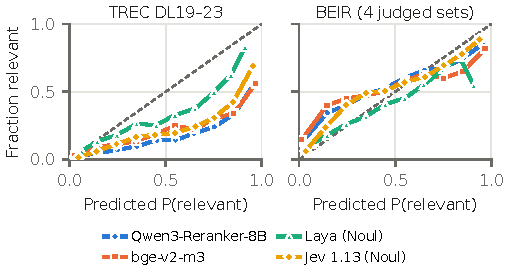
\includegraphics[width=\columnwidth]{figures/reliability.pdf}
\caption{Raw reliability on judged candidate pairs for bge, Qwen3-Reranker-8B, and the Noul readouts of Laya and Jev. Pooled within DL19--23 (left) and the four BEIR collections with negatives (right); 10 equal-width bins, hiding bins with fewer than 15 pairs. Noul needs no strict/lenient policy choice. Decision models are closer to the diagonal on DL; BEIR behavior is mixed.}
\label{fig:reliability}
\end{figure}

\paragraph{RQ2: Calibration.}
Raw cross-encoder scores were never meant to be probabilities, so we compare raw probabilities and probabilities after \emph{transfer} calibration, which uses no labels of the target collection (Table~\ref{tab:calibration}).
Jev and Laya's raw Noul probabilities improve calibration on judged candidate pools without target-label fitting. Jev Noul has mean ECE 5.0 points below bge (paired query-bootstrap 95\% CI $[-6.3,-3.9]$), lower on eight of nine collections, significantly lower on five after Holm, and significantly higher on none. TREC-COVID is slightly higher ($+0.17$). Laya Noul is 9.2 points lower ($[-10.8,-7.5]$). Jeff Noul is an exception: its ECE is 25.6 versus bge 20.0.
On DL, trained rerankers over-predict relevance (ECE 51.1/36.5/27.6 for Qwen0.6B/4B/8B, 47.0 for MiniLM, and 23.1 for bge; Figure~\ref{fig:reliability}).
For C3, the per-collection policy gives Jev a 5.1-point ECE advantage over bge ($[-7.1,-3.4]$), while strict everywhere gives $-0.7$ ($[-2.5,0.9]$). Jev's DBPedia ECE is worse by 9.9 under the policy and 14.1 under strict; Robust04 is worse by 0.9 under both.
These differences are insensitive to the number of bins (5--30) and to equal-mass binning (within 0.4 points). A Brier decomposition shows that Jev's advantage comes from both reliability (0.036 vs.\ 0.067 for Choice-3) and resolution (0.060 vs.\ 0.045).
Jev's Score-4 probabilities over-predict relevance under the per-collection policy (mean prediction 0.55 against a base rate of 0.31), because the lenient readout $P(\ell\ge1)$ counts ``related but not answering'' as relevant. Read strictly, they are better calibrated than bge-reranker-v2-m3 ($-2.1$, $[-3.4,-0.9]$).

Source-label transfer can give bge similar mean ECE. Pair-pooled transfer yields bge 14.9 and MiniLM 16.8, versus Jev C3/S4/Noul 9.1/8.2/14.2 and Laya C3 7.5. Collection-balanced pooling changes little.
Within-group transfer restricts sources by numeric binarization threshold and balances collections: DL$\to$DL and dense BEIR$\to$BEIR. This yields bge ECE 6.9, similar to Jev Noul 6.8, versus Jev C3 8.9 and Laya C3 9.3. The BEIR group mixes partial-relevance definitions with strict Robust04, so this is not identical semantic adaptation.
These descriptive means do not establish calibration equivalence; they show that source-label transfer can close the average raw-calibration gap on this suite.
On seven shared API collections, Clef C3 has raw ECE 7.8 and Brier 0.134 versus Jev C3 ECE 12.5 and bge 20.2. On three base-control collections, Clef Noul ECE is 13.1 versus its base 14.6, while C3 is 7.8. Jeff Noul ECE is 25.6 versus its base 26.5 across nine, and Jeff C3 is 15.3. These are configuration comparisons, not isolated training effects. Qwen235B's raw yes/no ECE is 20.5; transfer reduces it to 10.5 versus Jev Noul 13.0 on shared collections.
Calibration is conditional on judged candidates, whose mean base rate is 0.31. Treating unjudged candidates as negatives preserves the raw advantage of Jev Noul and Laya Noul, but reverses Jeff C3's advantage; Jeff Noul is worse already on judged pairs (Appendix Table~\ref{tab:judged}).

\paragraph{Efficiency.}
Per query--passage pair, the local cross-encoders and Qwen3-Reranker-0.6B take 0.3--14\,ms (median) on a laptop GPU, Qwen3-Reranker-4B and 8B 102 and 148\,ms (4-bit), Laya 58\,ms, and Jeff 100\,ms (with slow reference kernels); the API models take a median 176\,ms (Jev), 401\,ms (Clef), and 850\,ms (Qwen3-235B) per call with 8--24 concurrent requests. Reranking 100 passages costs \$3.4 per 1k queries with Jev on average (\$2.4--5.7; long documents cost more) and \$2.3 with the Qwen3-235B yes/no baseline; on the seven collections where both were run, Clef 27B costs about 4.8 times as much as Jev (\$15.3 vs.\ \$3.2).

\begin{table*}[t]
\centering
\footnotesize
\setlength{\tabcolsep}{4pt}
\caption{RQ3: answer F1 on the original 1{,}000 ID-disjoint final questions per dataset; MuSiQue component families overlap design splits. Avg.\ $n$: mean number of selected passages (independent of generator). $^\dagger$: Jev significantly better than bge-reranker-v2-m3 under the same policy in the original question-level paired $t$-test (Holm-corrected, $p<0.05$); these tests do not account for family dependence. Displayed policies and ranker-effect comparisons were fixed after separate pilot questions. Thresholds use a readout selected with labelled calibration questions; the $P>0.3$ rows are Platt-scaled.}
\label{tab:rag}
\begin{tabular}{lrrrrrrrr}
\toprule
 & \multicolumn{3}{c}{MuSiQue} & \multicolumn{3}{c}{NQ} & \multicolumn{2}{c}{Avg.\ $n$} \\
Policy & Qwen2.5-7B & Llama-3.1 & Qwen3-30B & Qwen2.5-7B & Llama-3.1 & Qwen3-30B & MuSiQue & NQ \\
\midrule
No context & 10.5 & 9.3 & 12.6 & 26.7 & 31.4 & 35.2 & 0.0 & 0.0 \\
All 20 passages & 38.8 & 37.0 & 46.3 & 52.5 & 49.4 & 51.5 & 20.0 & 20.0 \\
Gold passages (oracle) & 60.9 & 54.7 & 64.1 & 60.2 & 59.1 & 59.7 & 2.6 & 3.4 \\
\multicolumn{9}{l}{\textit{Jev 1.13}} \\
\quad top-1 & 45.2$^\dagger$ & 36.4$^\dagger$ & 43.4$^\dagger$ & 50.4 & 50.4$^\dagger$ & 51.4 & 1.0 & 1.0 \\
\quad top-3 & 44.6$^\dagger$ & 39.3$^\dagger$ & 47.1$^\dagger$ & 52.1 & 50.5 & 52.9 & 3.0 & 3.0 \\
\quad top-5 & 42.4$^\dagger$ & 40.7$^\dagger$ & 47.9$^\dagger$ & 51.9 & 50.9 & 53.0 & 5.0 & 5.0 \\
\quad adaptive-$k$ & 46.7$^\dagger$ & 40.2$^\dagger$ & 47.2$^\dagger$ & 52.3 & 50.1 & 52.3 & 2.9 & 6.2 \\
\quad $P>0.3$ & 43.6$^\dagger$ & 36.1$^\dagger$ & 43.5$^\dagger$ & 51.2 & 51.5 & 52.3 & 2.4 & 2.9 \\
\quad top-2 $+$ $P>0.3$ & 44.2$^\dagger$ & 39.1$^\dagger$ & 45.2$^\dagger$ & 51.8 & 51.0 & 53.2 & 3.0 & 3.5 \\
\multicolumn{9}{l}{\textit{bge-reranker-v2-m3}} \\
\quad top-1 & 22.0 & 18.0 & 23.7 & 47.9 & 47.1 & 49.1 & 1.0 & 1.0 \\
\quad top-3 & 38.5 & 31.5 & 39.1 & 51.4 & 50.5 & 52.6 & 3.0 & 3.0 \\
\quad adaptive-$k$ & 30.5 & 26.1 & 32.6 & 50.6 & 50.5 & 51.8 & 3.1 & 7.1 \\
\quad top-2 $+$ $P>0.3$ & 35.7 & 30.4 & 37.9 & 51.3 & 51.2 & 52.6 & 2.9 & 3.9 \\
\bottomrule
\end{tabular}
\end{table*}

\paragraph{RQ3: Context selection.}
Table~\ref{tab:rag} reports answer F1 on the original 1{,}000 ID-disjoint final questions per dataset; MuSiQue component families overlap design splits.
\emph{Ranking quality helps on the original multi-hop split.} On MuSiQue, passages selected by Jev beat those selected by bge-reranker-v2-m3 under every policy and with every generator, by $+2.6$ to $+23.2$ F1. All 27 comparisons pass the original question-level Holm tests (nine policies, three generators; Table~\ref{tab:rag} shows a subset), which assume independent questions despite family reuse. With Qwen2.5-7B, Jev's single top passage (45.2) or its Adaptive-$k$ selection of 2.9 passages (46.7) beats giving the generator all 20 candidates (38.8) with a small fraction of the generator input tokens. This saving excludes the cost of scoring all 20 candidates.
This coincides with a difference in \emph{which} passage each ranker puts first. bge-reranker-v2-m3's top passage is a supporting paragraph slightly more often (88.0\% vs.\ 82.2\%, McNemar $p<10^{-4}$), but usually the first hop---the one that shares the question's entities (61.9\%)---whereas Jev's top passage is the last, answer-bearing hop in 51.2\% of questions against 15.2\% ($p<10^{-80}$; Appendix Table~\ref{tab:ragsel}), and 56--64\% across Jev's three readouts.
Changing Qwen0.6B's instructions to relevant, answers, or contains the answer yields only 16.5--18.5\% last-hop@1 and 51--56\% first-hop@1. These tested wording changes do not reproduce Jev's preference, but do not establish its cause.
Replacing gold-answer strings with \texttt{[MASKED]} reduces Jev S4 last-hop@1 to 43.8\% (Noul: 50.3\%) versus unmasked 51.2\% (56.4\%); masked bge scores 13.4\%. This is a descriptive perturbation: the marker appears in 999 of 1,000 last-hop paragraphs but only 1,621 of 19,988 candidates, revealing answer location. Residual preference may use that cue, prior entity knowledge, or memorized chains; masking cannot isolate question resolution from these explanations.
On NQ, only one of the 27 ranker-effect comparisons is significant. The full downstream comparison is against bge; Qwen0.6B appears only in the selection diagnostic, and no RAG advantage over Qwen8B is established.
\begin{table}[t]
\centering\footnotesize\setlength{\tabcolsep}{3pt}
\caption{Retrospective MuSiQue sensitivity on 329 questions with no sub-question ID in calibration or pilot. Answer F1 under three ranker-effect policies; $\Delta$ is Jev minus bge. CIs resample 212 source-graph families (20,000 paired replicates, seed 13), retaining question weights; intervals are unadjusted. $^\dagger$: passes the original nine-policy question-level Holm correction (top-1 and Adaptive-$k$ for every generator; no top-3 comparison).}
\label{tab:rag-clean}
\begin{tabular}{llrrrr}
\toprule
Generator & Policy & Jev & bge & $\Delta$ & Family 95\% CI \\
\midrule
Qwen2.5-7B & top-1 & 41.8 & 23.1 & $+18.8^\dagger$ & $[14.0, 23.8]$ \\
 & Adaptive-$k$ & 42.1 & 31.3 & $+10.7^\dagger$ & $[5.9, 15.7]$ \\
 & top-3 & 43.6 & 41.3 & $+2.4$ & $[-2.6, 7.3]$ \\
\addlinespace[2pt]
Llama-3.1-8B & top-1 & 35.0 & 20.6 & $+14.4^\dagger$ & $[9.6, 19.2]$ \\
 & Adaptive-$k$ & 38.4 & 27.1 & $+11.3^\dagger$ & $[7.1, 15.7]$ \\
 & top-3 & 41.1 & 35.7 & $+5.5$ & $[1.0, 10.0]$ \\
\addlinespace[2pt]
Qwen3-30B-A3B & top-1 & 43.9 & 26.0 & $+17.9^\dagger$ & $[12.5, 23.4]$ \\
 & Adaptive-$k$ & 47.9 & 34.6 & $+13.3^\dagger$ & $[9.0, 17.8]$ \\
 & top-3 & 48.1 & 42.4 & $+5.7$ & $[0.8, 10.5]$ \\
\bottomrule
\end{tabular}
\end{table}

\emph{Retrospective component-clean sensitivity.} On the 329 questions with no sub-question ID directly shared with calibration or pilot, top-3 Jev/bge F1 is 43.6/41.3, 41.1/35.7, and 48.1/42.4 for Qwen2.5-7B, Llama-3.1-8B, and Qwen3-30B-A3B, respectively (Table~\ref{tab:rag-clean}). Gains shrink to $+2.4$, $+5.5$, and $+5.7$; none passes the original nine-policy question-level Holm correction. Family-bootstrap intervals are $[-2.6,7.3]$, $[1.0,10.0]$, and $[0.8,10.5]$, without multiplicity correction. Jev's point estimates remain higher under all nine shared policies ($+0.5$ to $+18.8$), and 14 of 27 original-style Holm tests pass, versus 27 on the full split. The passing tests include top-1 ($+14.4$ to $+18.8$) and Adaptive-$k$ ($+10.7$ to $+13.3$) for every generator, whose family-bootstrap intervals all exclude zero (Table~\ref{tab:rag-clean}); the gain shrinks most for top-3. The top-2+$P>0.3$ rule differs from Jev top-3 by $-1.5$, $+0.5$, and $-1.8$ F1; family intervals cross zero for every generator, as do comparisons with Adaptive-$k$. This sensitivity does not quantify overlap-induced inflation: subset size and case mix change. Moreover, 23 subset questions remain indirectly connected to design questions through other source records, so direct component exclusion does not establish full family isolation or absence of model-training contamination.
\emph{Thresholds on probabilities do not beat fixed $k$.} A pure threshold at 0.3 on Platt-scaled probabilities leaves the generator with no passage for 10.3\% of MuSiQue and 21.6\% of NQ questions, which then fall back to closed-book answering (the prompt does not allow abstention).
Raw $P>0.3$ on NQ is within 1.3 F1 of the Platt threshold and top-3 for every generator; on MuSiQue it selects nothing for 25\% and is 3.4--5.9 F1 below top-3. These post-hoc raw thresholds still use a readout chosen using labelled calibration questions (Appendix~\ref{app:extra}).
In a post-hoc equivalence analysis (TOST, $\pm2$ F1), the top-2+threshold rule is equivalent to top-2, top-3, top-5, and Adaptive-$k$ on NQ for every generator; on MuSiQue it is equivalent to top-2 (and, for Llama, to top-3), and pooled over generators it is 1.9 F1 below Adaptive-$k$ (95\% CI $[-3.4,-0.4]$; Holm-adjusted $p=0.065$). On MuSiQue it is also below Adaptive-$k$ for Qwen2.5-7B ($-2.6$) and below top-3 and top-5 for Qwen3-30B-A3B ($-1.9$, $-2.7$; unadjusted $p=0.01$--$0.05$, none significant after Holm), so ``equivalent or slightly worse'' is the fair summary. It selects exactly two passages for 61\% of MuSiQue and 55\% of NQ questions but more on the rest, 3.0 and 3.5 on average, so it saves no tokens over top-3.
On these data, Jev's practical advantage over bge is chiefly ranking; neither Platt-scaled nor calibration-selected raw thresholds establish improved context selection.
